\documentclass[12pt, english]{article}
%%%%%%%%%%%%%%%%%%%%%%%%%%%%%%%%%%%%%%%%%%%%%%%%%%%%%%%%

% margin %%%%%%%%%%%%%%%%%%%%%%
\usepackage{geometry}
 \geometry{
 a4paper,
 left=1in,
 top=0.9in,
 right=1in,
 bottom=2in,
 }
%%%%%%%%%%%%%%%%%%%%%%%%%%%%%%%%%%%%%%%%%%%%%%%%%%%%%%%%

% page no. %%%%%%%%%%%%%%%%%%%%%%
\usepackage{fancyhdr}
\pagestyle{fancy}
\fancyhf{}
\fancyfoot[C]{\textit{\thepage}}
\setlength{\headheight}{65pt}
%%%%%%%%%%%%%%%%%%%%%%%%%%%%%%%%%%%%%%%%%%%%%%%%%%%%%%%%

% idk-needed %%%%%%%%%%%%%%%%%%%%%%
\usepackage{amsmath,amsthm,amssymb,amsfonts, enumitem, color, comment, graphicx, environ, lipsum, accsupp}
%%%%%%%%%%%%%%%%%%%%%%%%%%%%%%%%%%%%%%%%%%%%%%%%%%%%%%%%

% code and color %%%%%%%%%%%%%%%%%%%%%%
\usepackage{spverbatim}
\usepackage{xcolor}
\usepackage{listings}
\definecolor{bluegrey}{RGB}{0, 0, 200}
\lstset{
        framexleftmargin=0pt,
        frame=shadowbox,
        rulesepcolor=\color{gray},
        xleftmargin=30pt,
        xrightmargin=30pt,
        breaklines=true,
        basicstyle=\ttfamily,
        showstringspaces=false,
        escapeinside={(*@}{@*)},
        }
\def\speciallstcolor{\begingroup\color{blue}}
\def\endspeciallstcolor{\endgroup}
%%%%%%%%%%%%%%%%%%%%%%%%%%%%%%%%%%%%%%%%%%%%%%%%%%%%%%%%

% heading %%%%%%%%%%%%%%%%%%%%%%
\renewcommand\thesection{\color{blue}\arabic{section}}
\newcommand{\mysection}[2]{\setcounter{section}{#1}\addtocounter{section}{-1}\section{#2}}
%%%%%%%%%%%%%%%%%%%%%%%%%%%%%%%%%%%%%%%%%%%%%%%%%%%%%%%%

% image %%%%%%%%%%%%%%%%%%%%%%%
\graphicspath{}
%%%%%%%%%%%%%%%%%%%%%%%%%%%%%%%%%%%%%%%%%%%%%%%%%%%%%%%%

% both side indent %%%%%%%%%%%%%%%%%%%%%%
\newenvironment{myindent}
{\par\leftskip25pt\relax\rightskip25pt\relax}
{\par\leftskip0cm\relax\rightskip0cm\relax}
%%%%%%%%%%%%%%%%%%%%%%%%%%%%%%%%%%%%%%%%%%%%%%%%%%%%%%%%

% type ^ and \ %%%%%%%%%%%%%%%%%%%%%%
\newcommand{\power}{$^\wedge$}
\newcommand{\backs}{\textbackslash} 
%%%%%%%%%%%%%%%%%%%%%%%%%%%%%%%%%%%%%%%%%%%%%%%%%%%%%%%%

% document info %%%%%%%%%%%%%%%%%%%%%%
\lhead{Arav Sarma \\ 15193845}  %replace with your name
\rhead{Homework \textcolor{blue}{9} \\ 2025 Speech Processing}
%%%%%%%%%%%%%%%%%%%%%%%%%%%%%%%%%%%%%%%%%%%%%%%%%%%%%%%%

% begin %%%%%%%%%%%%%%%%%%%%%%
\begin{document}
%wwwwwwwwwwwwwwwwwwwwwwwwwwwwwwwwwwwwwwwwwwwwwwwwwwwwwwwww

% section _______________________________________________
\mysection{9}{Creating the continua}
\vspace{10pt}

% -__-__-__-__-__-__-__-__-__-__-__-__-__-__-__-__-__-__-


% ><><><><><><><><><><><><><><><><><><><><><><><><><><><><><
\subsection*{\emph{2.} Written report}
\vspace{10pt}

\begin{itemize}
    \item \textbf{General research question:} \par
    Location of phoneme boundary as a function of lexical context (word-nonword)
    \item \textbf{Specific research question:} \par
    How does presence/absence of a lexical item effect categorisation of aspirated-breathy laryngeal contrast? Unlike the voicing or aspirated contrasts where boundary can be tested with VOT continua, the aspirated-breathy contrast would require manipulation of cues like turbulence quality and also pitch on following vowel (as the breathy and aspirated categories has been observed to effect pitch across languages; tonogenesis in Rohingya, Punjabi, tone-depressing effect in Southeastern Bantu, adaptation of indic loans with breathy in Thai). The study will look at lexical effect across this contrast for Assamese speakers from Guwahati.   
\end{itemize}

\paragraph{Methods}
\begin{itemize}
    \item \textbf{Participants} \par
    Recruited: \char`\~ 9 \\
    Tests completed: 0 \par
    Participants are going to be tested online using Zoom online meetings, and recruited through author's contacts, and likely by reaching out to Assam/Northeast related online forums like on reddit. The plan is to have Assamese speakers ideally all from Guwahati, this is to neutralise individual factors like regional variation, exposure to English. A different experiment setup can be by using a qualtrics form along with online meet, so the participants have more autonomy with the test and excess to stimuli on their device while also making it easier to see if they are in a quiet environment. \par
    \item \textbf{Continua}
    Continua from [dh] to [th]ː 1st context is with following segments [um], or [ila] (word to nonwordː dhum-*thum / dhila-*thila). 2nd context is with following segments [u] or [io] (nonword to word: *dhu-thu / *dhio-thio). \par
    \item \textbf{Duration} \par
    The breathy-aspirated contrast can involve duration of voicing, however the breathy phonation is not really the same as voicing of a vowel (vocal folds in breathy are not as / or not completely close together as in modal voice). Therefore it is amount of voicing (closeness of vocal folds) during the afterburst which would be contrastive cue in terms of voicing. The other place where duration might be important is onset of vowel (duration of afterbust). However this will not be a cue used for this study's continua as it has not been investigated if it is involved in breathy-aspirated contrast and because onset of vowel is not easy to determine, especially if some amount of voicing is present before the vowe which can be the case for breathy phonemes.  \par
    \item \textbf{Pitch} \par
    Pitch is a cue which will be used to form continua. The vowel portion of the sound will be manipulated for gradient (mean) pitch. To synthesise different pitches, first the target pitch points in the manipulation window are selected, then they are scaled up/down to desired mean pitch via \textbf{Multiply pitch frequencies...}. \par
    Points to consider:
    \begin{itemize}
        \item How is pitch gradient incorporated with degree of voicing gradient: congruent + non-congruent?
    \end{itemize}
    \item \textbf{Intensity} \par
    Intensity of voicing is a likely cue which will be manipulated for the continua. The portion of the sound concerned for this manipulation is the afterburst (turbulent region between the burst and onset of vowel). To simulate a breathy-aspirated afterburst different ratios of periodicity to aperiodicity need to be synthesised. 
\end{itemize} \par

\subsubsection*{Stimuli visualisations} 

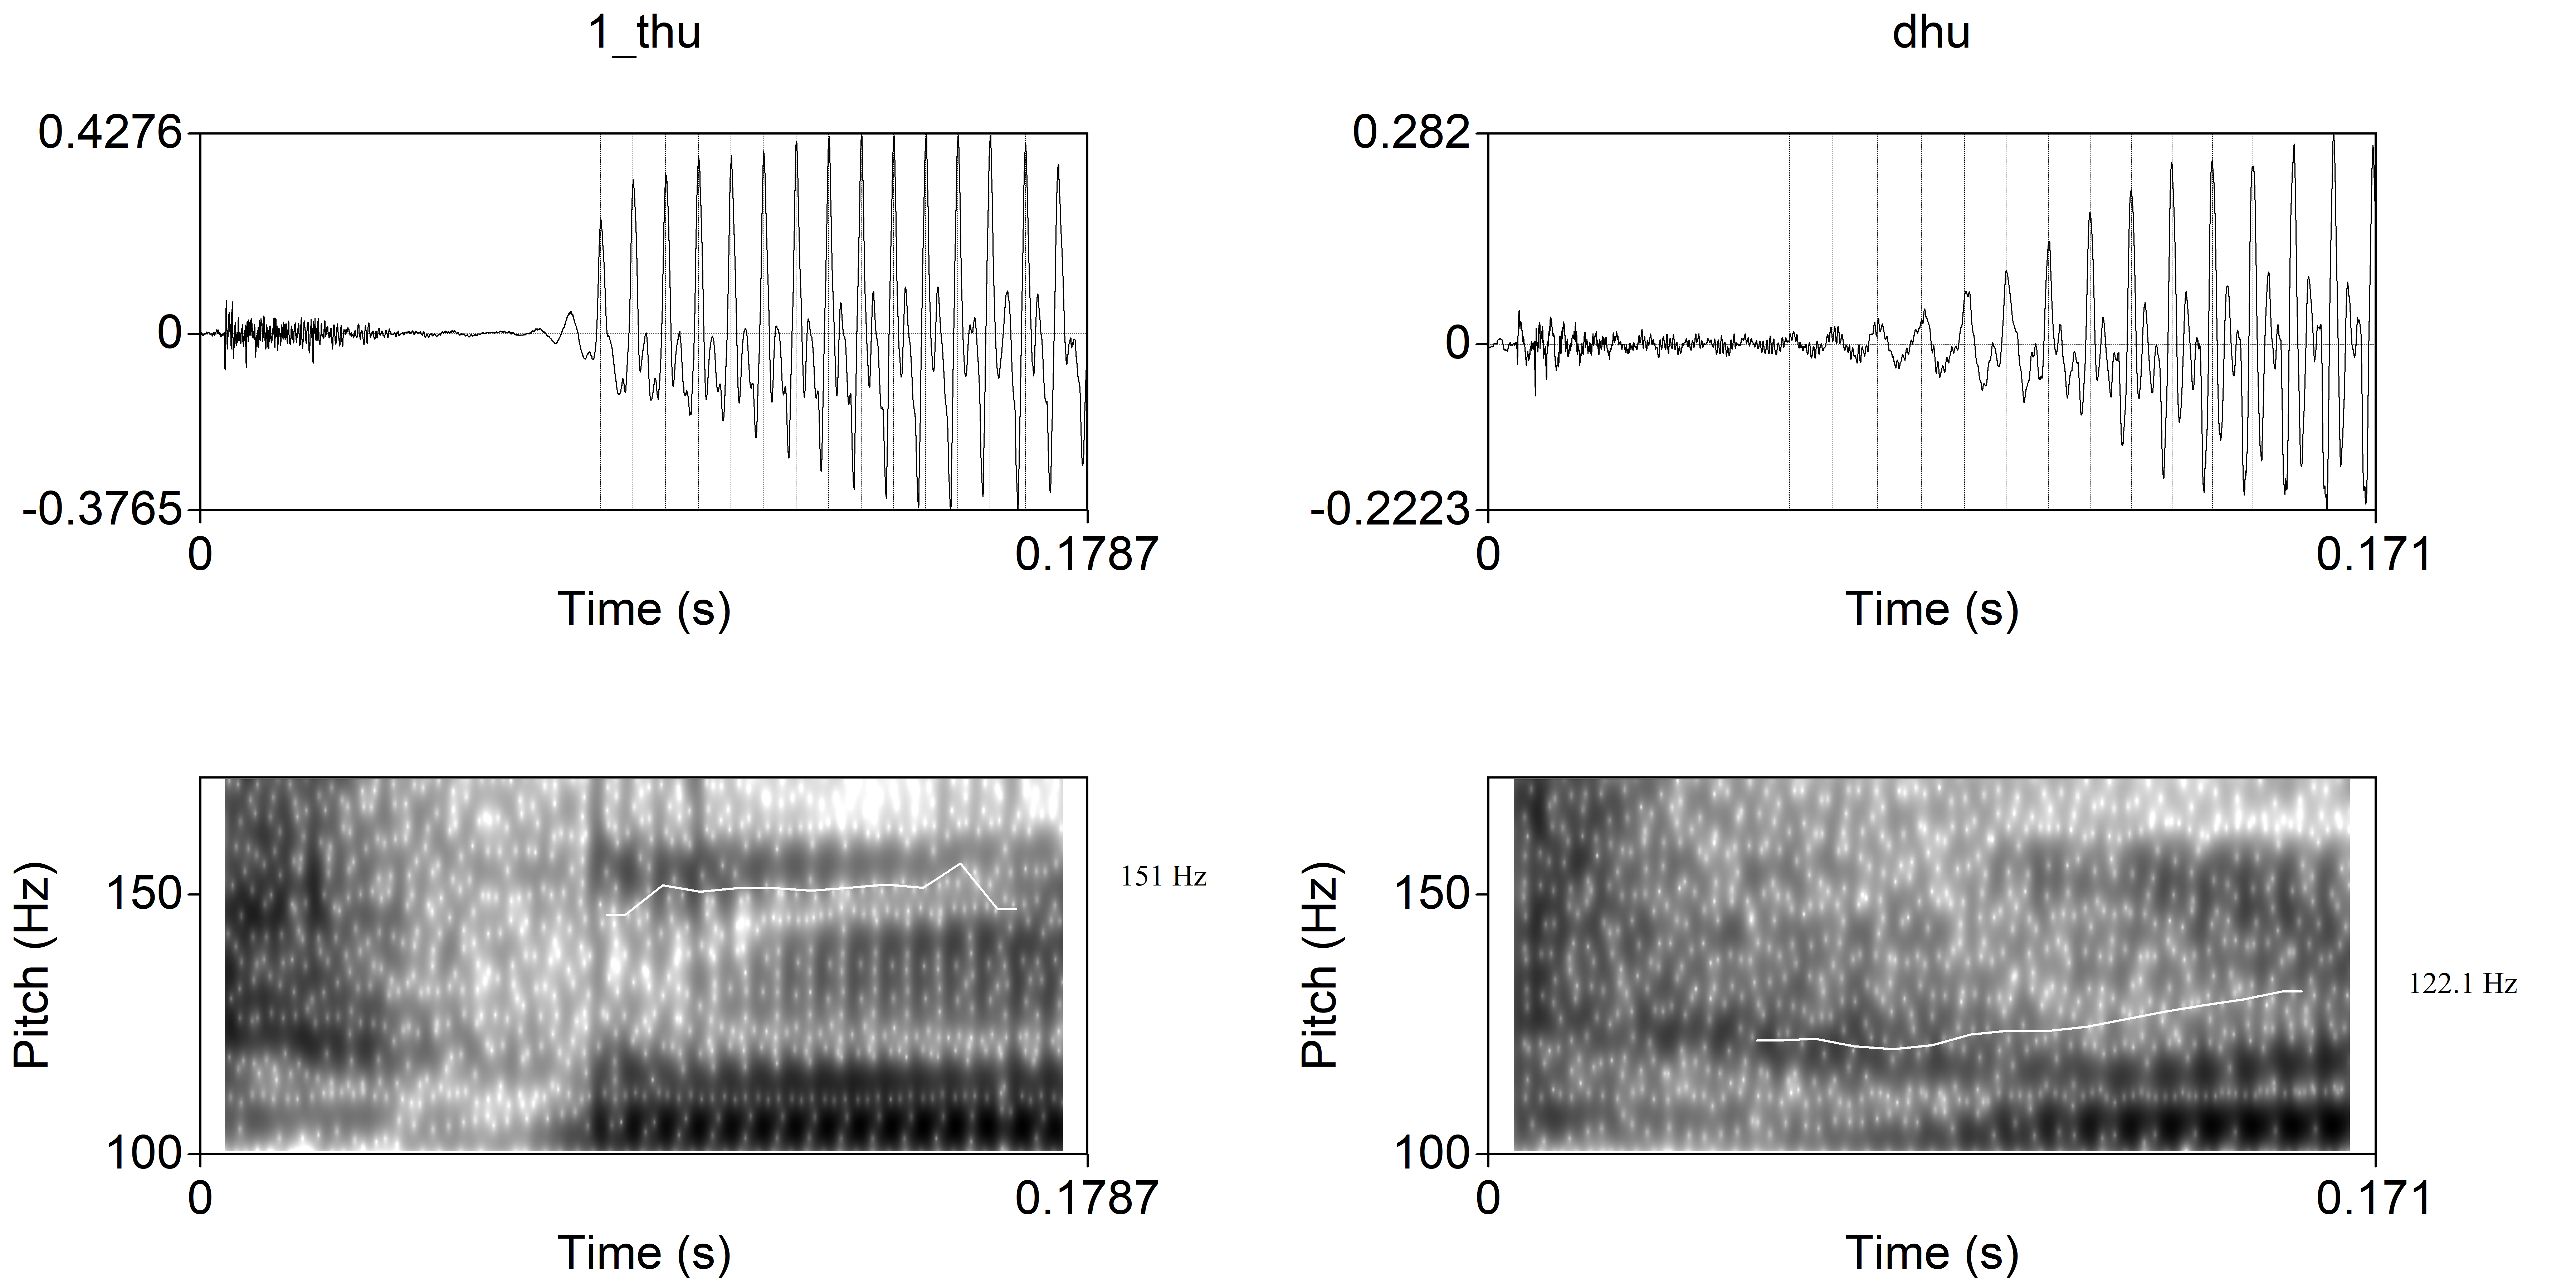
\includegraphics[scale=0.55]{thudhupraat.png} \par

Wave, pitch and spectograms for recorded /thu/ (also the aspirated endpoint token), and recorded /dhu/ (acoustic variant with gradual periodic transition).

\includegraphics[scale=0.5]{2-7praat.png} \par

Wave, pitch and spectograms of synthesised samples for aspirated to breathy continuum.
\vspace{25pt}

To synthesize voicing during afterburst to vowel transition like the recorded /dhu/ sample, a sine wave was created using the formula:

\[ 0.03 \cdot sin(2 \cdot pi \cdot 124.34 \cdot x) \cdot 2^\frac{x}{0.015} + randomGauss(0, 0.007) \]

\[ 0.02 \cdot sin(2*pi \cdot 124.341 \cdot x) \cdot 2^\frac{x}{0.015} + 0.01 \cdot sin (2*pi \cdot 1809.54 \cdot x) \cdot 2^\frac{-x}{0.02} + randomGauss(0, 0.002) \]

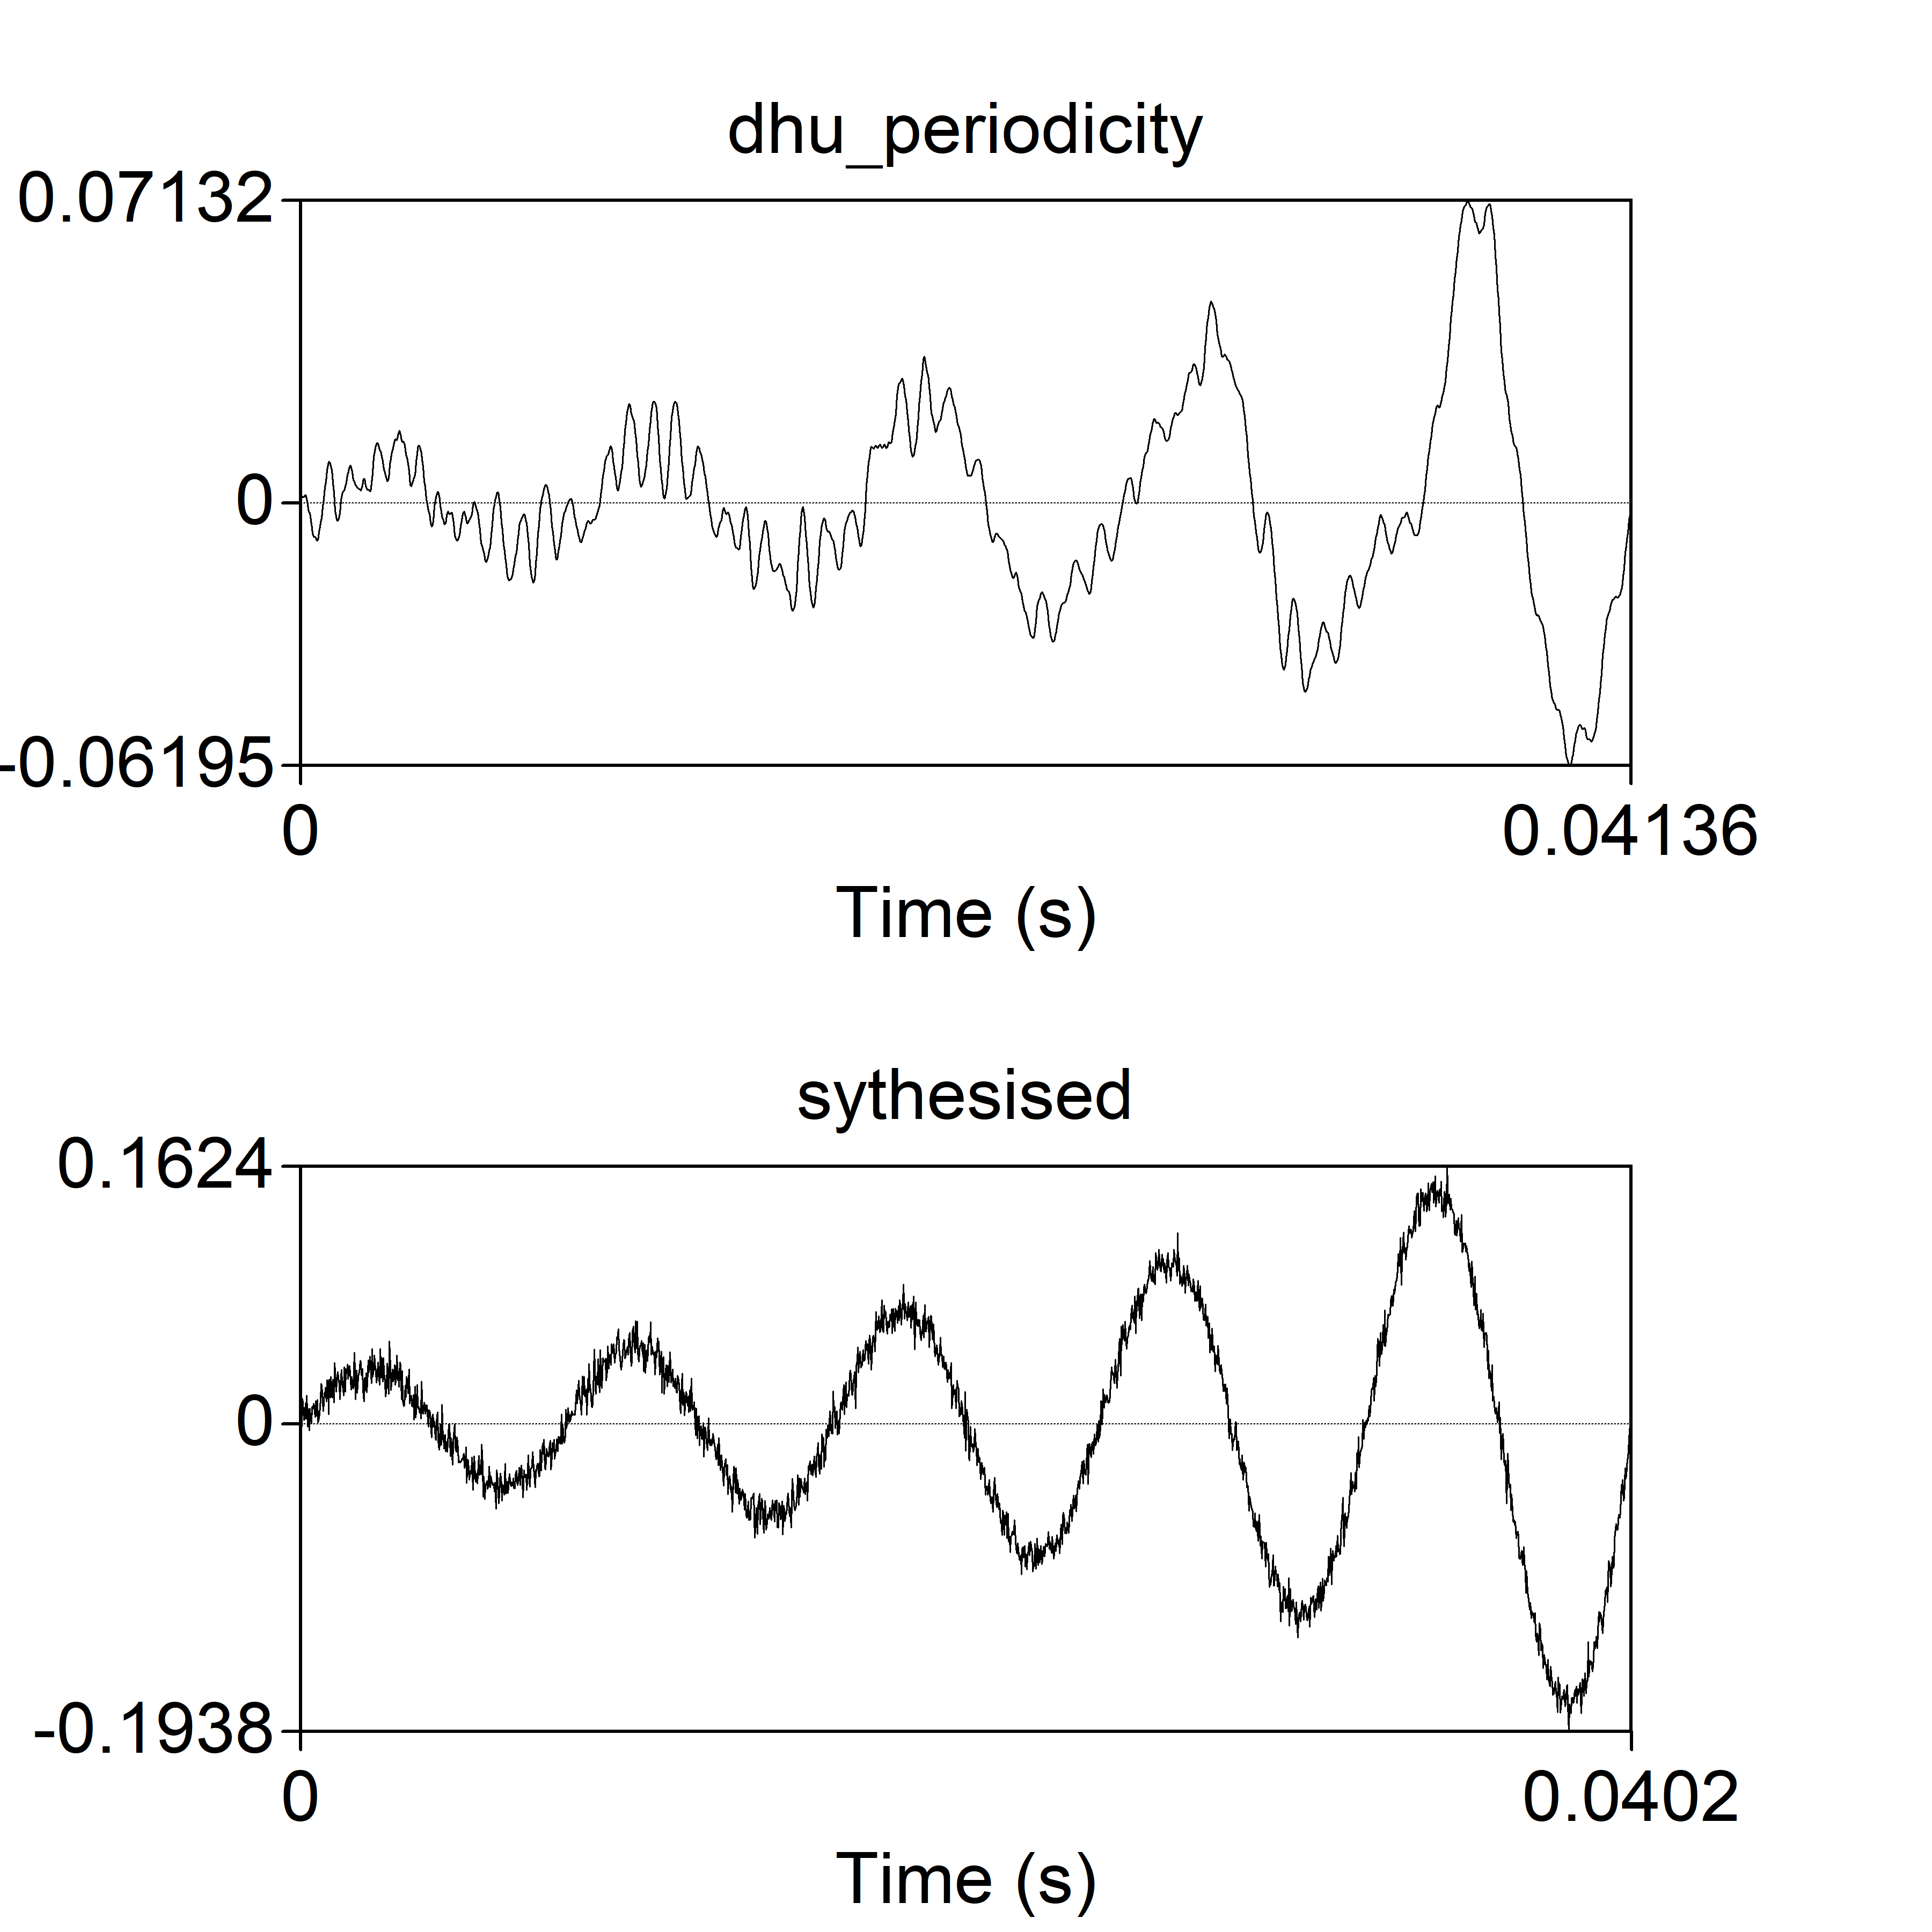
\includegraphics[]{afterburstpraat.png} \par

Waveforms for periodicity during afterburst to vowel transition in /dhu/ (top), and sample 7.

\subsubsection*{Creation of continuum (needs to be updated)}

\begin{itemize}
    \item dhu (right) to thu continuum
    \begin{itemize}
        \item First manipulation object is created from the sound. Pitch points before the selected region in praat picture are removed.
        \item The endpoint tokens have pitches 126.2 Hz (dhu) and 152.7 Hz (thu). For 5 tokens in between the pitch needs to be increased (152.7-126.2) / 5 = 5.3 Hz in each step.
        \item Before increasing for the next step, the manipulated sound needs to be created using publish resynthesis.
    \end{itemize}  
\end{itemize}

% ><><><><><><><><><><><><><><><><><><><><><><><><><><><><><


%wwwwwwwwwwwwwwwwwwwwwwwwwwwwwwwwwwwwwwwwwwwwwwwwwwwwwwwww
\end{document}